\section{Base Class Reference}
\label{classBase}\index{Base@{Base}}
Inheritance diagram for Base:\begin{figure}[H]
\begin{center}
\leavevmode
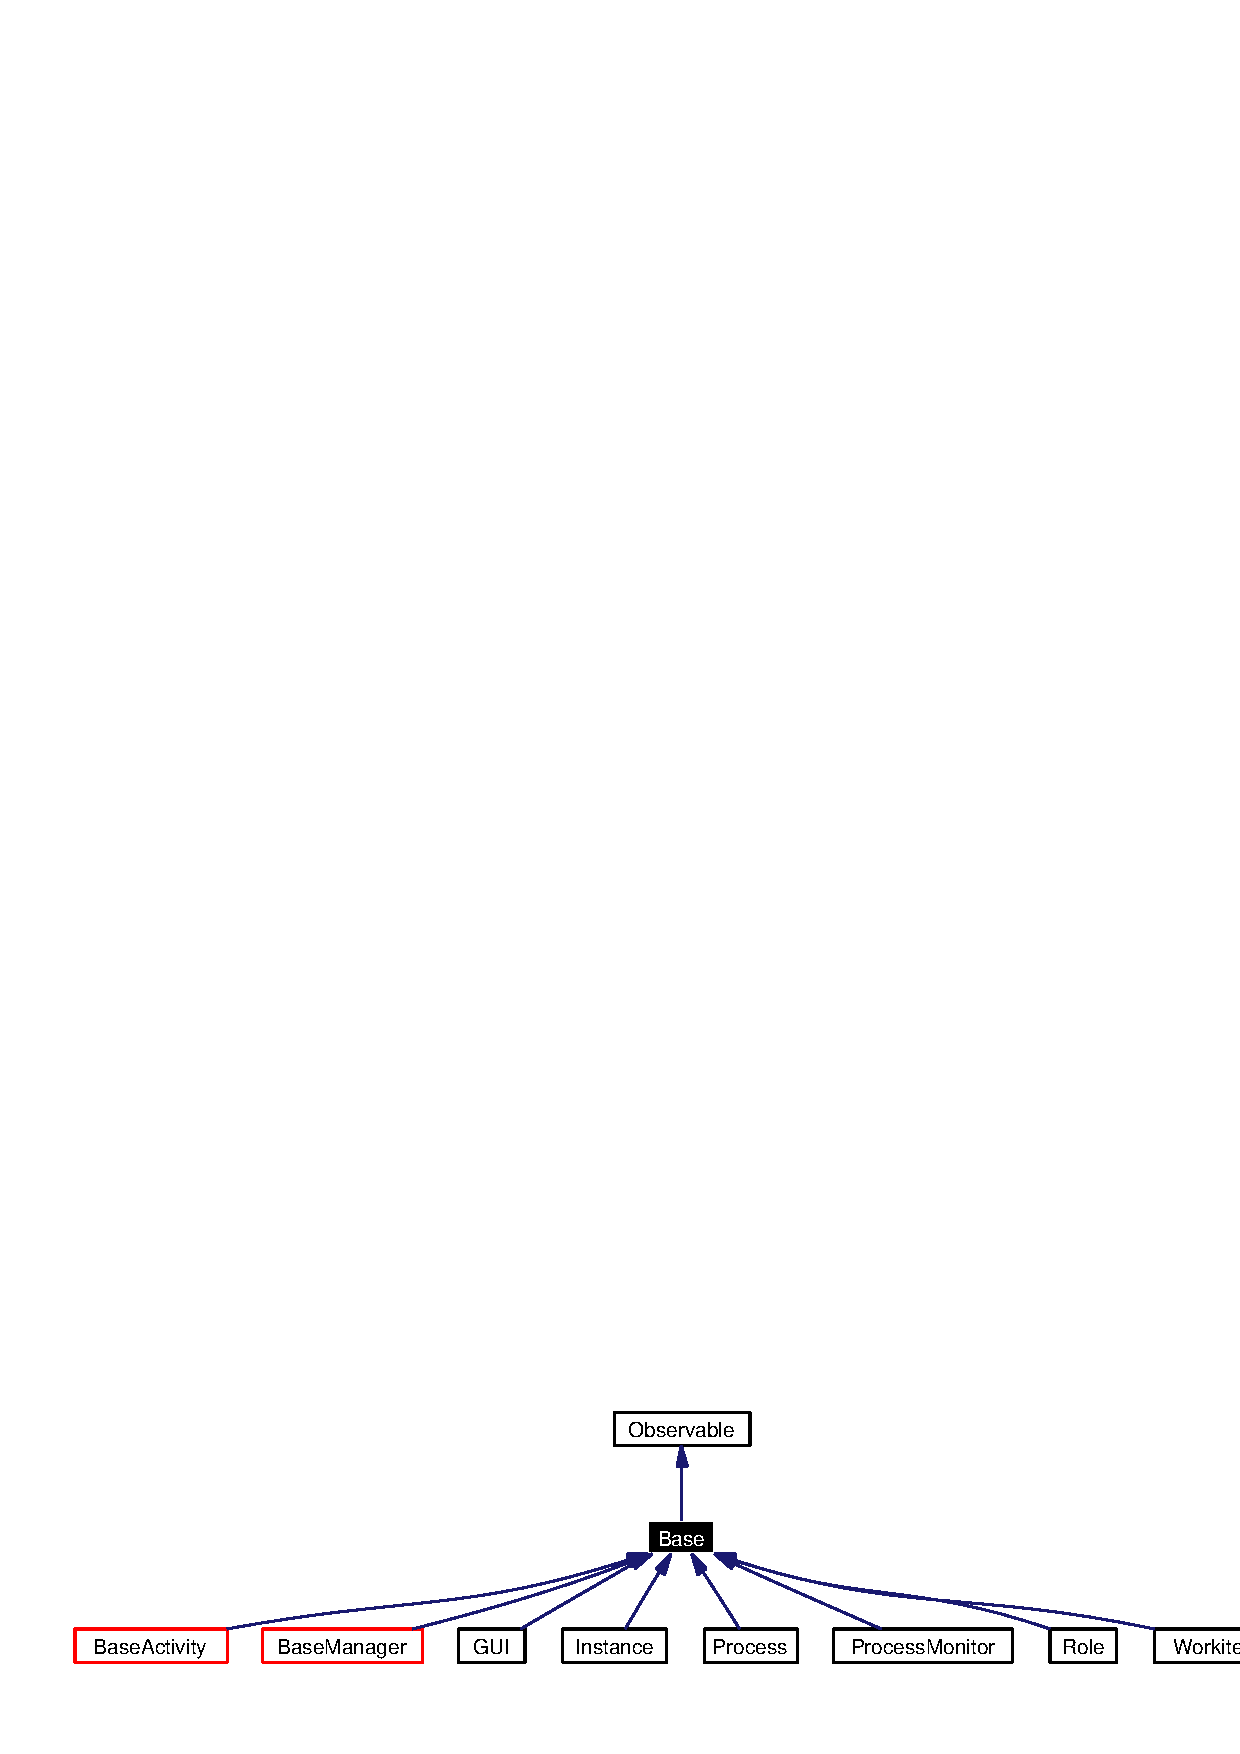
\includegraphics[width=307pt]{classBase__inherit__graph}
\end{center}
\end{figure}
Collaboration diagram for Base:\begin{figure}[H]
\begin{center}
\leavevmode
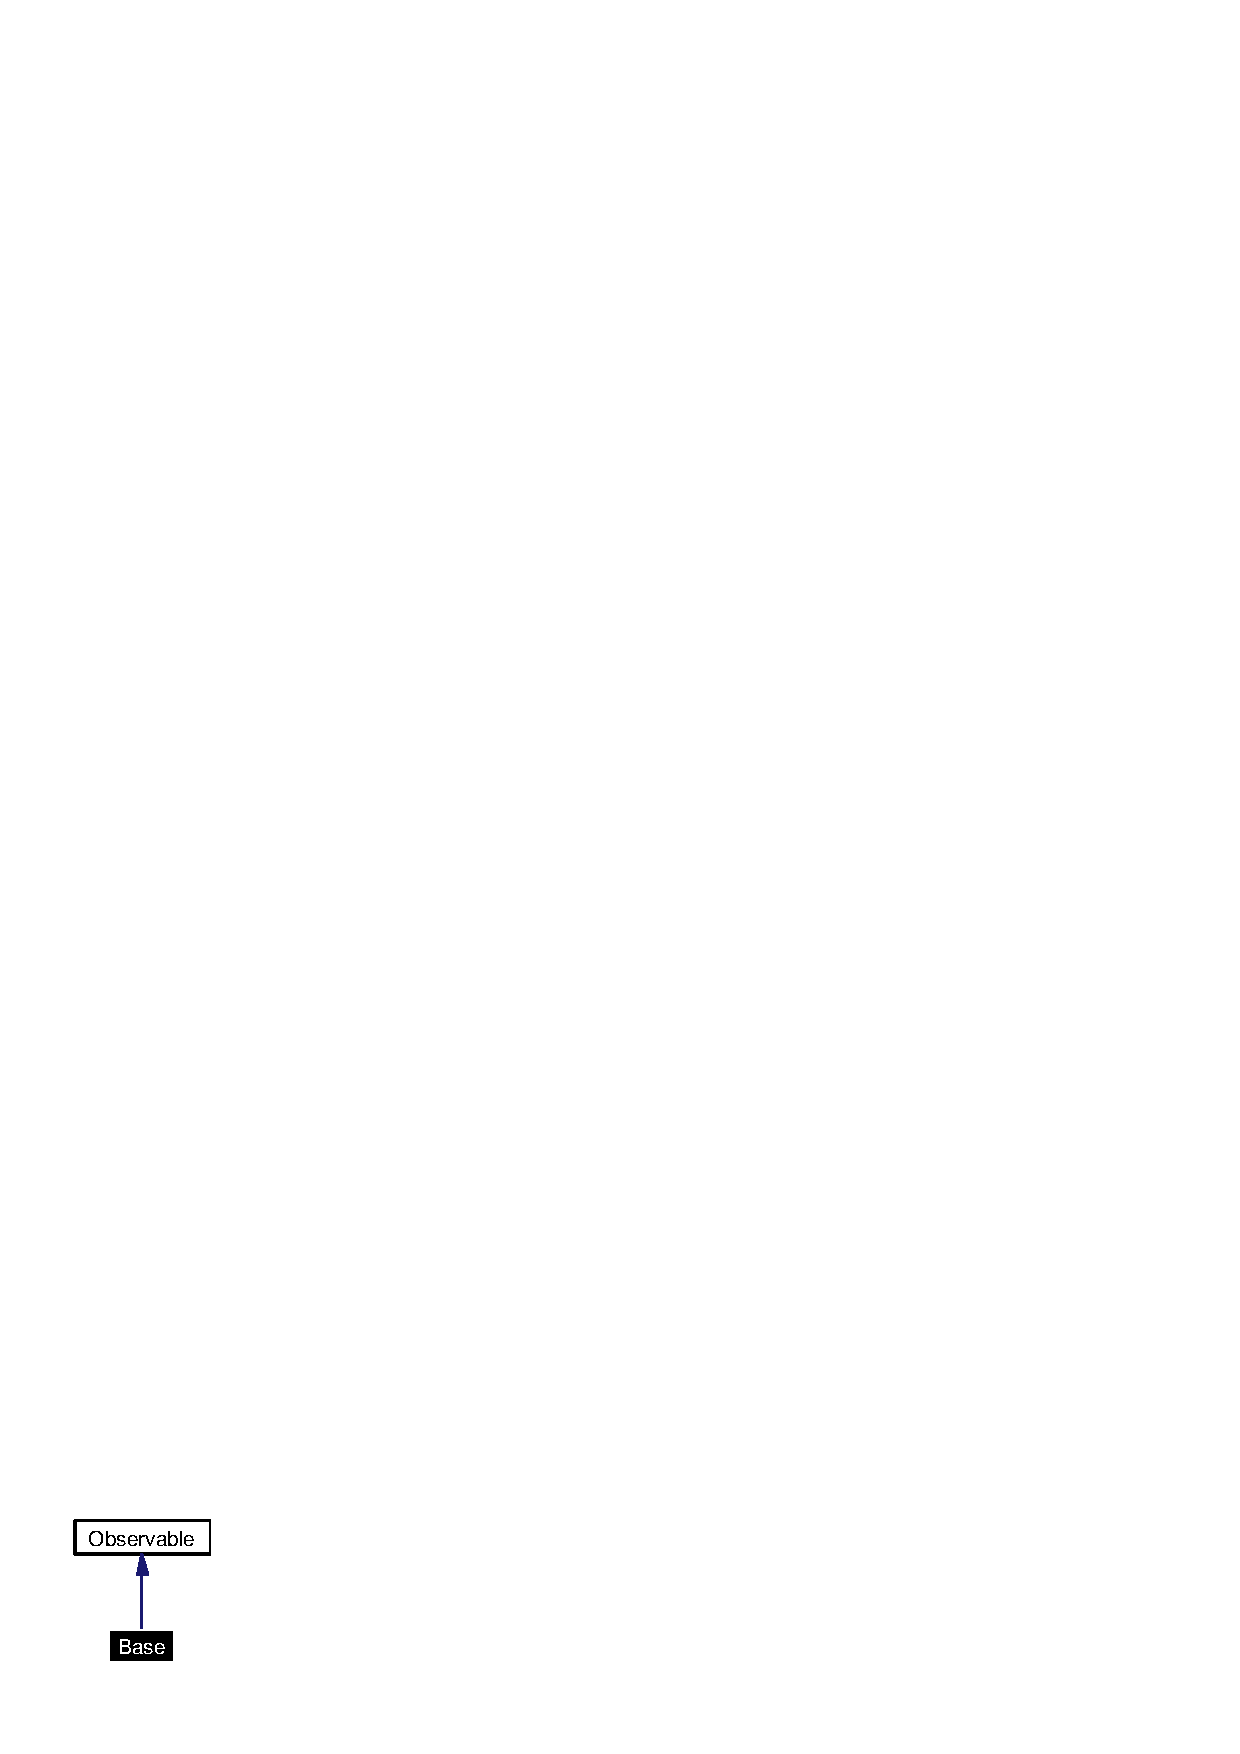
\includegraphics[width=50pt]{classBase__coll__graph}
\end{center}
\end{figure}
\subsection*{Public Member Functions}
\begin{CompactItemize}
\item 
{\bf Base} (\$db)\label{classBase_a0}

\item 
{\bf query} (\$query, \$values=null, \$numrows=-1, \$offset=-1, \$reporterrors=true)\label{classBase_a1}

\item 
{\bf get\-One} (\$query, \$values=null, \$reporterrors=true)\label{classBase_a2}

\item 
{\bf sql\_\-error} (\$query, \$values, \$result)\label{classBase_a3}

\item 
{\bf convert\_\-query} (\&\$query)\label{classBase_a4}

\item 
{\bf convert\_\-sortmode} (\$sort\_\-mode)\label{classBase_a5}

\item 
{\bf convert\_\-binary} ()\label{classBase_a6}

\end{CompactItemize}
\subsection*{Public Attributes}
\begin{CompactItemize}
\item 
{\bf \$db}\label{classBase_o0}

\item 
{\bf \$num\_\-queries} = 0\label{classBase_o1}

\end{CompactItemize}


\subsection{Detailed Description}
This class is derived by all the API classes so they get the database connection, database methods and the {\bf Observable}{\rm (p.\,\pageref{classObservable})} interface. 



Definition at line 9 of file Base.php.

The documentation for this class was generated from the following file:\begin{CompactItemize}
\item 
Base.php\end{CompactItemize}
